\documentclass[tikz,border=3.14pt]{standalone}
\usetikzlibrary{arrows.meta}
% Reconstructed as editable vector paths; no embedded reference bitmap.
% Coordinates are in original-image pixels, with the origin at the upper left.
% Compile: pdflatex -output-directory=tmp mwe.tex
% Ten rendered comparison rounds are archived in tmp/iteration-01 ... iteration-10.
% Blue dimensions are restored in the final scope, after the illustration.
% The real kite string, blue shoes, and navy kite knot are intentionally retained.
% This is a vector approximation: raster blur and compression are not reproduced.
\definecolor{leaf}{RGB}{169,208,79}
\definecolor{leafedge}{RGB}{96,110,57}
\definecolor{bark}{RGB}{232,195,159}
\definecolor{barkedge}{RGB}{132,112,85}
\definecolor{band}{RGB}{240,169,107}
\definecolor{skin}{RGB}{239,186,130}
\definecolor{ink}{RGB}{99,91,67}
\definecolor{hair}{RGB}{71,71,71}
\definecolor{hairline}{RGB}{56,57,53}
\definecolor{shirt}{RGB}{252,247,191}
\definecolor{shorts}{RGB}{250,73,37}
\definecolor{shortedge}{RGB}{139,59,35}
\definecolor{shoe}{RGB}{42,105,142}
\definecolor{shoeedge}{RGB}{48,81,88}
\definecolor{pink}{RGB}{221,122,177}
\definecolor{cyan}{RGB}{136,209,223}
\definecolor{kiteedge}{RGB}{84,87,82}
\definecolor{knot}{RGB}{47,54,126}
\definecolor{string}{RGB}{159,153,135}
\def\TreeWidth{1.20}
\def\BoyWidth{1.20}
\def\KiteWidth{1.15}
\def\StringWidth{1.15}
\def\TreeX{0}
\def\TreeY{0}
\def\BoyX{0.20}
\def\BoyY{-0.16}
\begin{document}
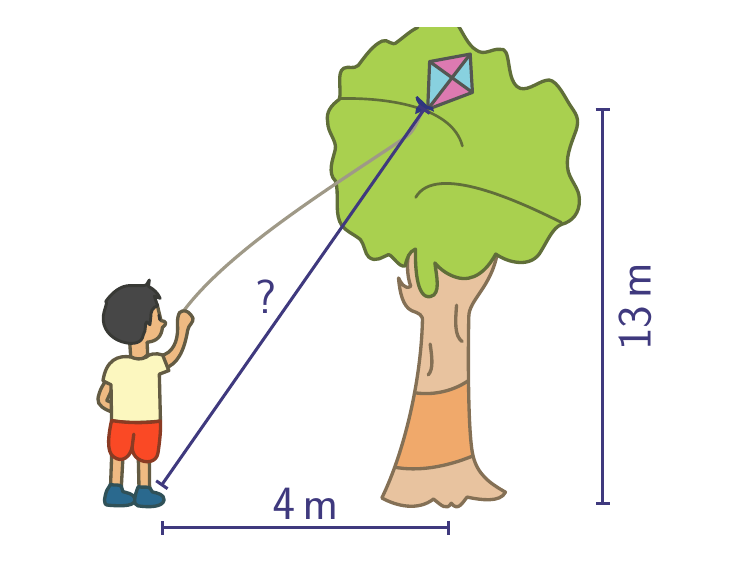
\begin{tikzpicture}[x=1bp,y=-1bp,line cap=round,line join=round]
  \path[use as bounding box] (0,0) rectangle (243,185);
  \clip (0,0) rectangle (243,185);
  % Tree trunk, lower orange band, roots, and bark creases.
  \begin{scope}[shift={(\TreeX,\TreeY)},line width=\TreeWidth bp]
    % Share one trunk silhouette: clip the band, then stroke the outline once.
    \def\TrunkOutline{
      (137.8,78.7)
      .. controls (136.3,83.2) and (136.4,89.0) .. (137.9,93.1)
      .. controls (135.7,94.5) and (134.2,91.6) .. (133.5,90.1)
      .. controls (134.0,95.7) and (135.1,100.4) .. (138.3,101.9)
      .. controls (140.7,102.8) and (142.5,103.3) .. (142.1,106.0)
      .. controls (141.5,127.6) and (135.5,152.9) .. (127.5,169.3)
      .. controls (132.9,172.3) and (140.6,174.0) .. (146.1,169.7)
      .. controls (149.0,172.0) and (150.8,174.0) .. (152.5,171.2)
      .. controls (155.0,174.4) and (156.6,170.8) .. (158.2,169.0)
      .. controls (162.9,170.0) and (170.2,171.1) .. (172.0,167.2)
      .. controls (166.1,163.9) and (162.0,160.7) .. (160.4,154.4)
      .. controls (158.5,147.4) and (158.5,119.0) .. (158.8,104.2)
      .. controls (158.7,98.0) and (166.9,93.6) .. (169.1,81.0)
      -- cycle}
    \path[fill=bark] \TrunkOutline;
    \begin{scope}
      \clip \TrunkOutline;
      % Extend the band beyond both sides so it cannot create a second edge.
      \path[fill=band,draw=barkedge]
        (120.0,127.936) -- (138.5,131.3)
        .. controls (145.1,132.5) and (152.6,131.2) .. (158.6,127.1)
        -- (180.0,112.477) -- (180.0,146.082) -- (160.2,154.2)
        .. controls (150.2,158.3) and (140.3,159.8) .. (132.0,158.2)
        -- (120.0,155.887) -- cycle;
    \end{scope}
    \draw[draw=barkedge] \TrunkOutline;
    \draw[draw=barkedge] (154.4,99.9)
      .. controls (154.0,105.3) and (153.5,110.9) .. (156.4,113.0);
    \draw[draw=barkedge] (144.9,113.9)
      .. controls (145.5,118.3) and (146.2,122.9) .. (144.2,125.0);
    % Crown outline: irregular lobes, including the small hanging central leaf.
    \path[fill=leaf,draw=leafedge]
      (112.2,25.8)
      .. controls (113.1,22.5) and (111.1,16.0) .. (113.8,14.6)
      .. controls (115.6,13.7) and (117.3,15.1) .. (119.0,13.6)
      .. controls (121.5,10.3) and (124.3,6.2) .. (127.7,4.8)
      .. controls (129.6,3.8) and (131.1,7.1) .. (133.1,5.1)
      .. controls (136.0,2.9) and (138.1,1.0) .. (140.2,0.0)
      .. controls (140.2,-2.7) and (151.8,-4.0) .. (154.8,-1.1)
      .. controls (156.6,1.7) and (158.6,6.4) .. (161.4,8.0)
      .. controls (164.4,10.3) and (167.0,7.5) .. (170.0,7.8)
      .. controls (174.3,6.7) and (172.0,17.7) .. (176.2,21.2)
      .. controls (179.0,23.7) and (183.6,19.6) .. (186.5,19.0)
      .. controls (189.8,17.7) and (192.7,23.7) .. (195.0,27.5)
      .. controls (197.2,31.0) and (199.1,32.4) .. (197.2,37.6)
      .. controls (195.4,42.4) and (193.5,47.0) .. (194.6,51.7)
      .. controls (195.6,55.4) and (198.6,58.0) .. (198.6,61.7)
      .. controls (198.9,66.8) and (195.9,69.9) .. (192.2,70.8)
      .. controls (189.0,72.1) and (187.2,76.6) .. (184.9,80.3)
      .. controls (181.6,86.7) and (173.2,84.8) .. (168.5,81.5)
      .. controls (165.3,87.4) and (160.5,91.7) .. (154.4,89.9)
      .. controls (151.6,89.1) and (148.9,87.4) .. (146.6,84.7)
      .. controls (147.1,89.2) and (148.9,96.0) .. (145.0,96.8)
      .. controls (139.9,97.8) and (139.5,86.0) .. (139.6,79.7)
      .. controls (137.3,80.6) and (136.5,83.0) .. (135.9,85.8)
      .. controls (133.6,86.4) and (131.4,81.9) .. (129.9,81.7)
      .. controls (127.9,82.4) and (125.4,84.7) .. (122.8,82.6)
      .. controls (121.4,81.4) and (121.2,78.0) .. (119.8,76.3)
      .. controls (117.4,74.2) and (113.6,73.1) .. (112.3,69.7)
      .. controls (110.6,65.5) and (112.2,59.5) .. (110.8,55.2)
      .. controls (107.8,52.3) and (109.9,47.3) .. (110.7,44.0)
      .. controls (111.5,40.8) and (107.9,37.8) .. (108.0,33.9)
      .. controls (107.3,30.4) and (109.3,27.9) .. (112.2,25.8) -- cycle;
    \draw[draw=leafedge,line width=0.95bp]
      (112.8,25.5) .. controls (128.1,25.2) and (152.7,27.9) .. (156.5,42.6);
    \draw[draw=leafedge,line width=1.00bp]
      (139.7,61.1) .. controls (146.8,48.5) and (177.3,62.7) .. (192.1,70.1);
  \end{scope}
  % Actual kite string, separate from the straight dimension guide below.
  \draw[draw=string,line width=\StringWidth bp]
    (55.8,102.44) .. controls (72.9,79.1) and (115.0,53.9) .. (136.8,38.9)
    .. controls (139.6,36.5) and (140.6,32.5) .. (143.0,28.4);
  % Kite: four alternating fabric panels, frame, and tied blue knot.
  \begin{scope}[shift={(0.11,0.11)},line width=\KiteWidth bp,draw=kiteedge]
    \path[fill=cyan] (144.6,12.1) -- (159.2,9.4) -- (160.0,23.2) -- (143.9,29.3) -- cycle;
    \path[fill=pink,draw=none] (144.6,12.1) -- (159.2,9.4) -- (152.5,18.0) -- cycle;
    \path[fill=pink,draw=none] (152.5,18.0) -- (160.0,23.2) -- (143.9,29.3) -- cycle;
    \draw (144.6,12.1) -- (159.2,9.4) -- (160.0,23.2) -- (143.9,29.3) -- cycle;
    \draw (144.6,12.1) -- (160.0,23.2);
    \draw (159.2,9.4) -- (143.9,29.3);
    \path[fill=knot,draw=none] (143.8,28.0) -- (140.2,24.5)
      .. controls (138.6,24.4) and (140.2,27.6) .. (141.8,28.5)
      .. controls (139.3,27.6) and (139.7,29.5) .. (139.4,31.0)
      -- (143.9,29.1) -- (146.2,30.2) -- (145.7,28.5) -- cycle;
  \end{scope}
  % Boy, back-to-front: arms, legs, face, clothes, shoes, hair.
  \begin{scope}[shift={(\BoyX,\BoyY)},draw=ink,line width=\BoyWidth bp]
    \path[fill=skin,draw=ink] (29.0,126.8)
      .. controls (27.4,127.1) and (25.4,131.2) .. (25.1,133.8)
      .. controls (24.8,136.1) and (27.6,137.6) .. (30.0,138.5)
      -- (31.1,135.5) -- (28.3,134.4) -- (30.7,129.2) -- cycle;
    \path[fill=skin,draw=ink] (47.3,118.4)
      .. controls (52.3,117.4) and (53.8,112.9) .. (53.8,108.2)
      .. controls (53.5,105.8) and (53.9,102.1) .. (55.4,102.2)
      .. controls (57.2,101.7) and (58.3,103.0) .. (59.3,104.7)
      .. controls (59.7,106.2) and (57.6,107.3) .. (57.4,109.1)
      .. controls (56.1,117.0) and (53.4,121.4) .. (49.5,122.6) -- cycle;
    \path[fill=skin,draw=ink] (30.1,152.5) -- (34.2,152.9) -- (33.5,165.8)
      -- (29.6,165.9) -- cycle;
    \path[fill=skin,draw=ink] (39.6,153.9) -- (43.6,153.9) -- (43.7,166.7)
      -- (39.9,166.8) -- cycle;
    \path[fill=skin,draw=ink] (36.3,110.2) -- (36.9,118.7)
      .. controls (38.4,121.1) and (41.6,119.5) .. (43.0,117.9)
      -- (42.8,113.4)
      .. controls (46.3,113.1) and (48.0,111.3) .. (48.3,108.1)
      .. controls (50.0,106.9) and (49.9,105.8) .. (47.8,105.6)
      -- (46.4,99.8) -- (39.7,99.7) -- cycle;
    \path[fill=shirt,draw=ink] (36.9,118.7)
      .. controls (32.3,118.0) and (28.0,119.8) .. (26.9,127.3)
      -- (29.8,128.7) -- (30.0,141.6)
      .. controls (35.4,142.7) and (42.3,142.3) .. (47.6,141.8)
      -- (47.2,124.9) -- (50.6,123.6) -- (48.4,118.0)
      .. controls (46.1,117.1) and (43.2,117.7) .. (42.6,118.7)
      .. controls (40.5,119.8) and (38.8,119.5) .. (36.9,118.7) -- cycle;
    \path[fill=shorts,draw=shortedge] (30.0,141.6)
      .. controls (35.6,142.5) and (42.0,142.6) .. (47.6,141.8)
      .. controls (47.8,145.3) and (47.2,150.1) .. (46.7,153.3)
      .. controls (46.2,156.7) and (42.2,157.2) .. (39.6,155.4)
      .. controls (38.2,154.6) and (37.5,153.0) .. (37.4,151.2)
      .. controls (36.7,154.8) and (33.7,156.9) .. (30.8,154.7)
      .. controls (27.8,152.9) and (29.1,145.6) .. (30.0,141.6) -- cycle;
    \draw[draw=shortedge] (37.4,151.2) -- (38.0,146.5);
    \path[fill=shoe,draw=shoeedge] (29.6,164.6)
      .. controls (31.2,165.1) and (32.5,164.4) .. (33.5,165.3)
      -- (34.1,167.2)
      .. controls (35.2,167.5) and (38.2,168.0) .. (38.4,169.7)
      .. controls (38.8,172.4) and (34.5,172.5) .. (29.0,172.1)
      .. controls (26.4,172.1) and (27.7,168.8) .. (28.2,166.9) -- cycle;
    \path[fill=shoe,draw=shoeedge] (39.6,165.4)
      .. controls (41.1,165.9) and (43.0,165.1) .. (43.9,166.0)
      -- (44.7,167.3)
      .. controls (46.6,167.7) and (49.0,168.2) .. (48.9,170.2)
      .. controls (48.5,172.8) and (43.5,172.9) .. (39.5,172.3)
      .. controls (37.5,172.1) and (38.4,168.2) .. (39.6,165.4) -- cycle;
    \path[fill=hair,draw=hairline,line width=1.05bp] (43.6,91.0)
      -- (43.3,93.3)
      .. controls (45.1,94.3) and (46.6,95.5) .. (47.5,97.6)
      -- (45.4,96.8) -- (46.6,100.3)
      .. controls (44.8,100.7) and (44.0,102.4) .. (44.1,104.6)
      -- (43.8,107.1) -- (42.7,106.1)
      .. controls (41.7,106.5) and (42.7,108.9) .. (41.4,110.8)
      .. controls (41.0,113.9) and (37.6,114.1) .. (35.2,113.6)
      .. controls (31.1,112.9) and (27.3,109.8) .. (27.0,105.5)
      .. controls (26.7,103.6) and (27.8,101.1) .. (28.2,99.3)
      -- (27.9,98.7)
      .. controls (30.4,95.3) and (33.2,93.1) .. (36.5,93.0)
      .. controls (38.8,92.9) and (41.1,93.3) .. (42.5,92.8) -- cycle;
    \draw[draw=hairline,line width=0.95bp] (47.0,103.6) -- (47.3,105.3);
  \end{scope}

  % Dimensions: named anchors + orthogonal projections + shared Bar tips.
  % Method reference: https://tex.stackexchange.com/q/767109 (cfr's answer).
  \begin{scope}[
    dimension/.style={draw=dimensionblue,line width=1.1bp,
      {Bar[width=5bp]}-{Bar[width=5bp]}},
    every node/.style={text=dimensionblue,font=\sffamily\fontsize{16}{19}\selectfont,
      inner sep=0pt,outer sep=0pt}
  ]
    \definecolor{dimensionblue}{RGB}{63,57,126}
    \coordinate (dim-foot) at (48,165);
    \coordinate (dim-kite) at (143,29);
    \coordinate (dim-base) at (152,180);
    \coordinate (dim-height) at (207,172);

    \draw[dimension] (dim-foot) -- (dim-kite)
      node[midway,left=6bp] {?};
    \draw[dimension] (dim-foot |- dim-base) -- (dim-base)
      node[midway,above=3bp] {4\,m};
    \draw[dimension] (dim-height) -- (dim-height |- dim-kite)
      node[midway,sloped,below=6bp] {13\,m};
  \end{scope}
\end{tikzpicture}
\end{document}
